% Source: TeX Live 2025, doc/generic/pgf/pgfmanual-en-tikz-plots.tex:733-764
% (ybar interval and xbar interval): same unequal bin edges, units and sample
% magnitudes, except the horizontal bars point left and both final values
% are deliberate sentinels. Six coordinates give FIVE bars in each series.
% pgfmanual-en-library-plot-handlers.tex:424-434,442-490 gives the relative
% centers and widths: red occupies each bin's first half; teal its last half.
% Neither the final red height -4 nor the final teal length +6 is painted.
\documentclass[border=2pt]{standalone}
\usepackage{tikz}
\begin{document}
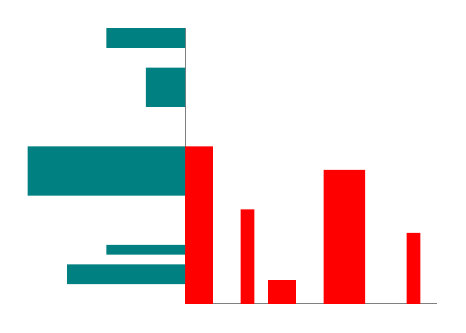
\begin{tikzpicture}
  \draw[gray] (0,3.5) -- (0,0) -- (3.2,0);
  \begin{scope}[x=10pt]
    \fill[red,bar interval width=0.5,bar interval shift=0.25] plot[ybar interval]
      coordinates {(0,2) (2,1.2) (3,0.3) (5,1.7) (8,0.9) (9,-4)};
  \end{scope}
  \begin{scope}[x=0.5cm,y=0.5cm]
    \fill[teal,bar interval width=0.5,bar interval shift=0.75] plot[xbar interval]
      coordinates {(-3,0) (-2,1) (-4,1.5) (-1,4) (-2,6) (6,7)};
  \end{scope}
\end{tikzpicture}
\end{document}
